\section{Methodology}

This section describes the dataset construction process, image preprocessing pipeline, feature extraction techniques, and classification models used for herbal plant recognition.

\subsection{Dataset Construction}

The dataset used in this study was constructed from 21 video clips containing different herbal plant species captured under diverse environmental and lighting conditions. The videos were processed frame-by-frame to extract representative images for classification. Since consecutive video frames often contain redundant information, only frames satisfying predefined quality criteria were retained.

After preprocessing and filtering, a total of 425 images were obtained and organized into 14 plant classes labeled from A to N. To ensure reproducibility and unbiased evaluation, the dataset was divided into training, validation, and testing subsets using stratified sampling.

The final dataset split consisted of:

\begin{itemize}
\item Training set: 297 images (70\%)
\item Validation set: 64 images (15\%)
\item Test set: 64 images (15\%)
\end{itemize}

\begin{table}[t]
\centering
\caption{Dataset statistics showing the number of preprocessed plant images per pseudo-label class (A through N).}
\label{tab:dataset_stats}
\begin{tabular}{lc@{\hspace{4em}}lc}
\toprule
\textbf{Class} & \textbf{Image count} & \textbf{Class} & \textbf{Image count} \\
\midrule
A & 11 & H & 30 \\
B & 43 & I & 9  \\
C & 27 & J & 16 \\
D & 37 & K & 38 \\
E & 33 & L & 40 \\
F & 34 & M & 47 \\
G & 29 & N & 31 \\
\midrule
\textbf{Total} & & & \textbf{425} \\
\bottomrule
\end{tabular}
\end{table}


\subsection{Image Preprocessing}

The raw video frames exhibited considerable variability in image quality, vegetation coverage, illumination, and background content. To improve dataset consistency, a preprocessing pipeline was developed consisting of vegetation filtering, blur detection, image normalization, and data augmentation.

% Figure 1: Examples of herbal plant images from different classes
\begin{figure}[t]
  \centering
  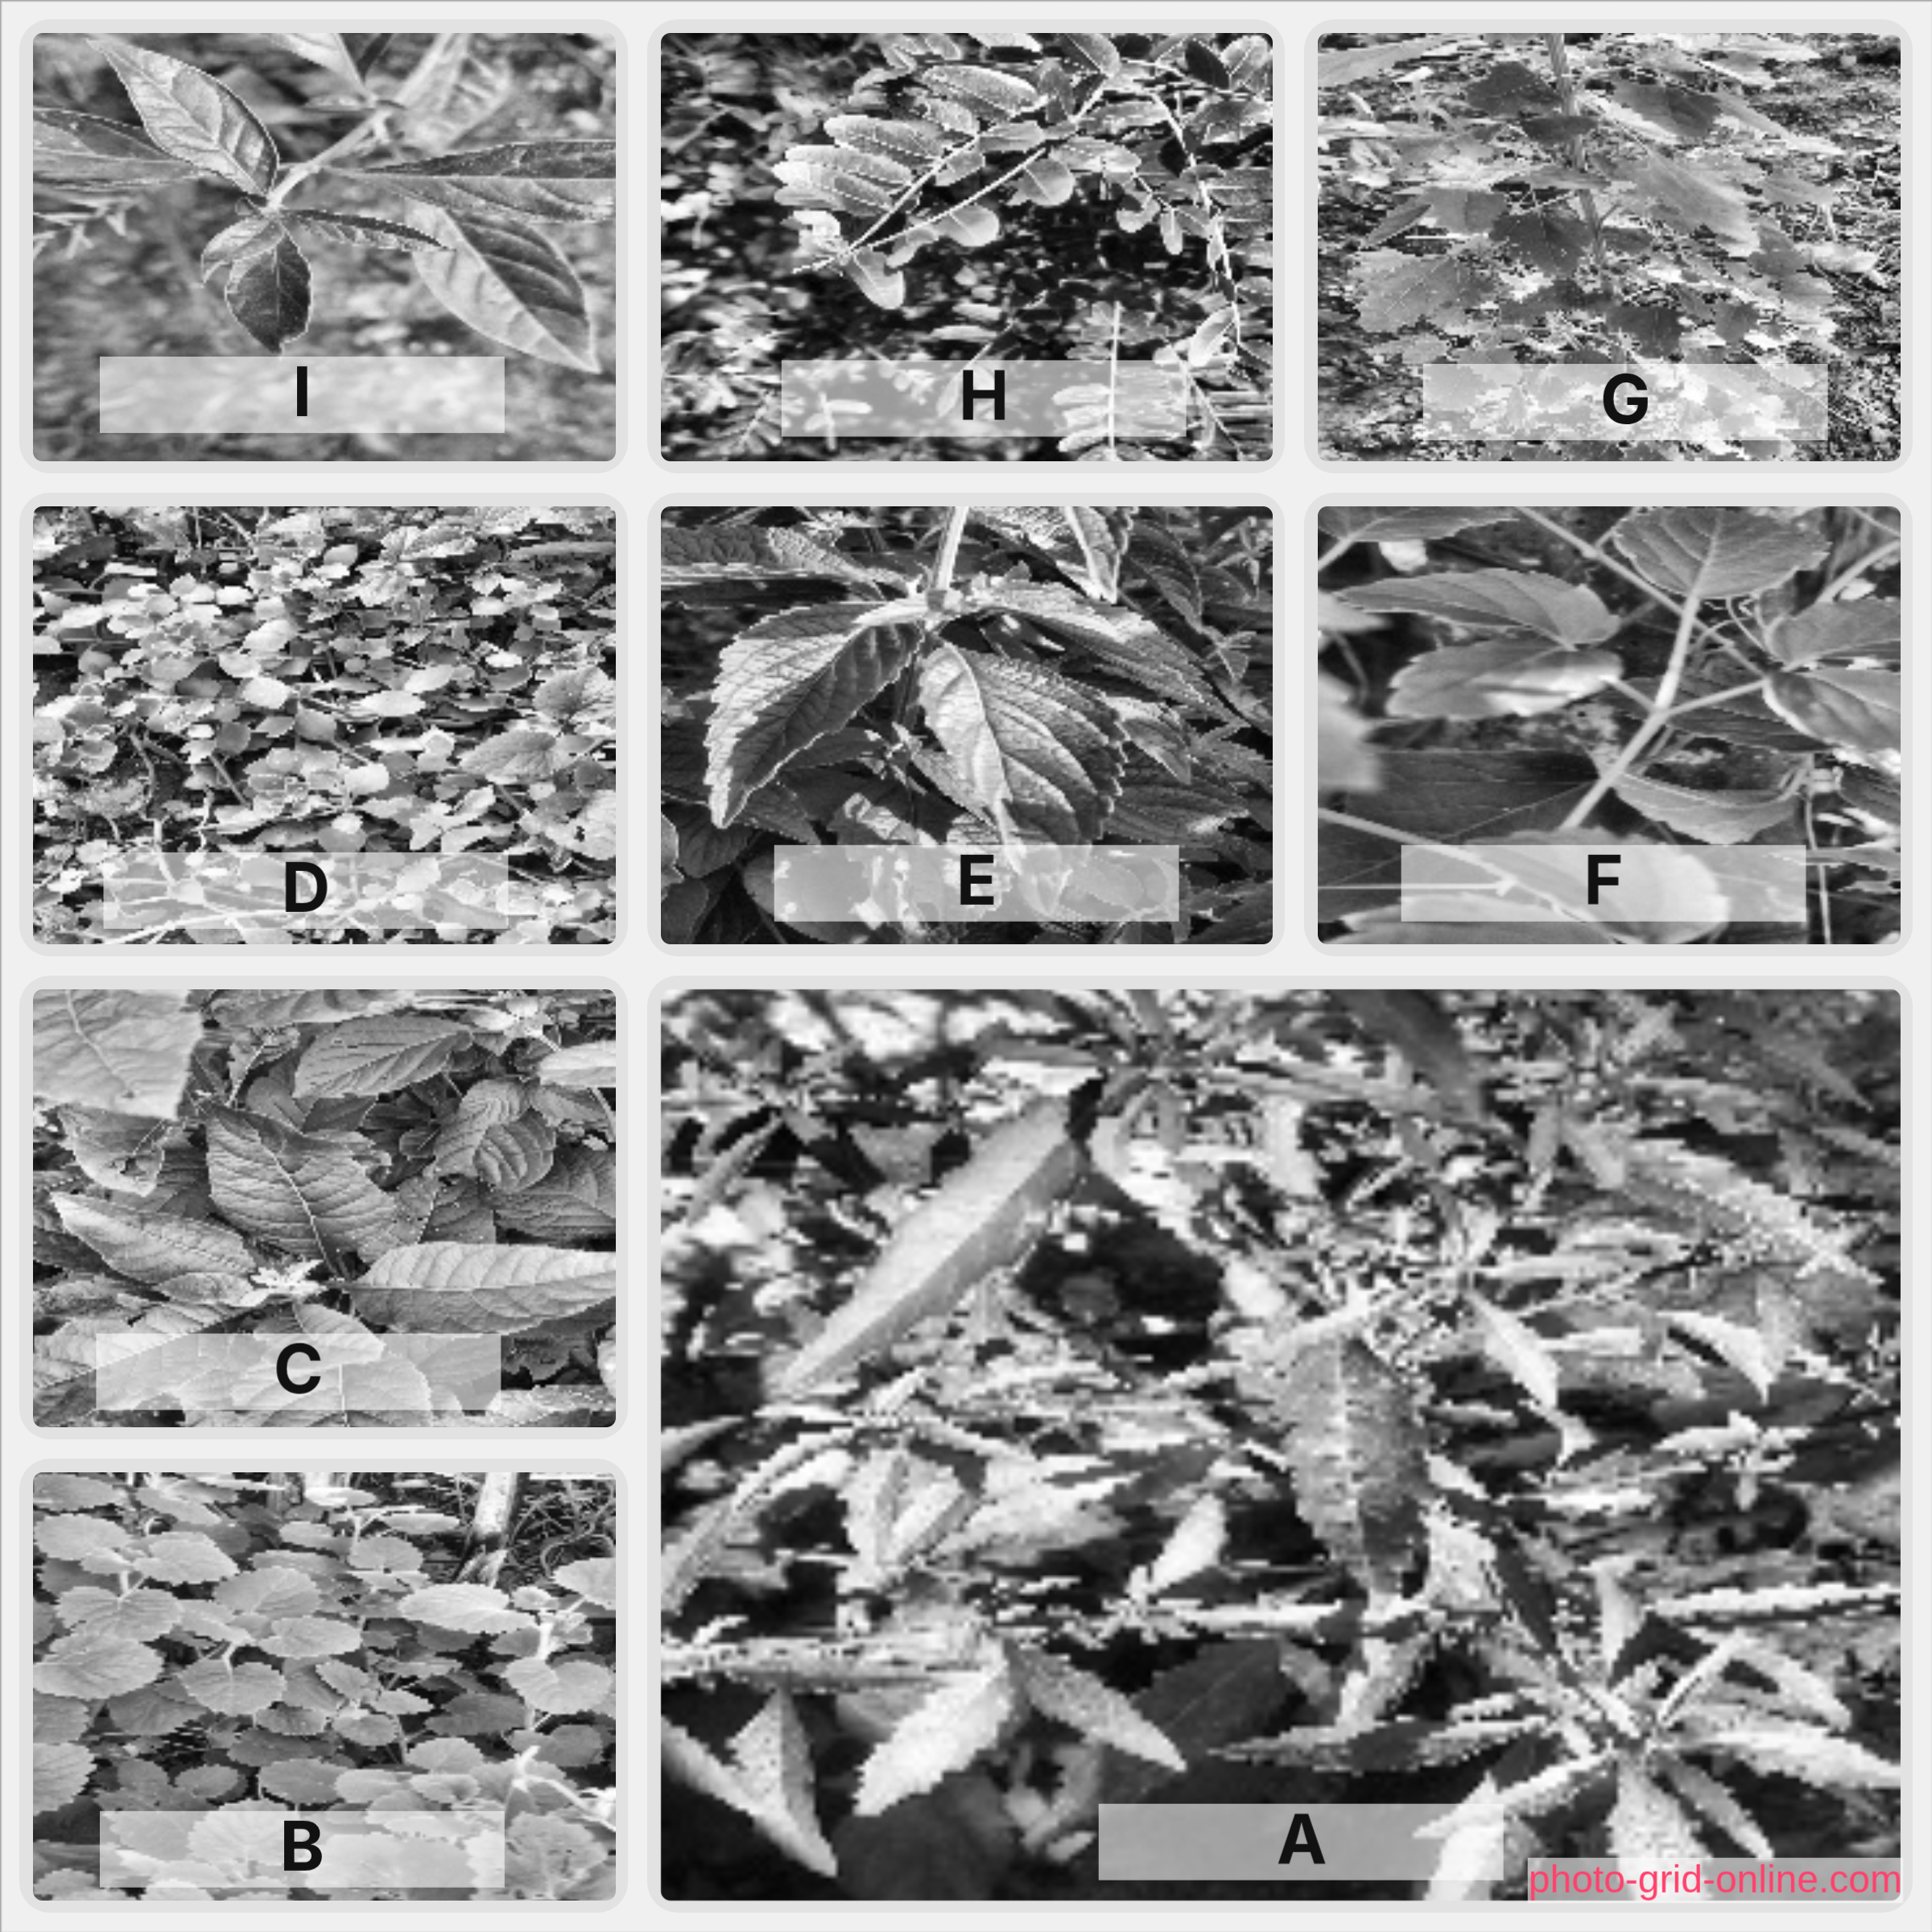
\includegraphics[width=\linewidth]{media/samples.png}
  \caption{Examples of herbal plant images from different classes}
  \label{fig:samples}
\end{figure}

\subsubsection{Vegetation Filtering}

Since the objective was to classify herbal plants, images containing insufficient vegetation were removed. Vegetation regions were identified using color thresholding in the HSV color space. Green pixels corresponding to plant regions were detected and their proportion within the image was computed.

Images containing less than a predefined vegetation coverage threshold were discarded. This step reduced the inclusion of frames dominated by background objects and improved the relevance of the training data.

% Figure 2: Vegetation filtering process showing original image, mask, and filtered output

\subsubsection{Blur Detection}

Video frames often contain motion blur caused by camera movement or plant motion. To eliminate low-quality samples, image sharpness was evaluated using the Variance of Laplacian method.

The Laplacian operator measures high-frequency image content associated with edges and texture. Images with variance values below a predefined threshold were considered blurry and excluded from the dataset.

This filtering process improved the quality of the extracted visual features and reduced noise during model training.

% Figure 3: Example of accepted and rejected images based on blur detection

\subsubsection{Image Normalization}

All retained images were resized to a uniform resolution of $224 \times 224$ pixels. For deep learning experiments, pixel intensities were normalized to the range $[0,1]$ to facilitate stable optimization during training.

\subsubsection{Data Augmentation}

To increase dataset diversity and reduce overfitting, data augmentation was applied during training. Each image was subjected to random transformations including:

\begin{itemize}
\item Horizontal flipping
\item Rotation between $-20^\circ$ and $20^\circ$
\item Brightness adjustment
\item Gaussian blurring
\end{itemize}

These transformations simulate real-world variations in plant appearance and improve model generalization.

% Figure 4: Examples of augmented images generated from a single frame

\subsection{ORB Feature Extraction and Bag-of-Visual-Words Representation}

The traditional machine learning pipeline employed Oriented FAST and Rotated BRIEF (ORB) descriptors to capture local image features. ORB was selected because it provides computational efficiency while maintaining robustness to rotation and scale variations.

For each image, up to 1000 ORB keypoints were detected and corresponding descriptors were extracted. The descriptors collected from all training images were combined to form a feature pool containing 232,788 local descriptors.

To convert variable-length descriptor sets into fixed-length feature vectors, a Bag-of-Visual-Words (BoVW) representation was adopted. MiniBatch K-Means clustering was applied to the descriptor pool to construct a visual vocabulary consisting of 500 visual words.

Each image was then represented as a normalized histogram describing the frequency of occurrence of each visual word.

% Figure 5: ORB keypoints and Bag-of-Visual-Words pipeline
% INSERT FIGURE HERE

\subsection{Traditional Machine Learning Classifiers}

The BoVW feature vectors were used to train four traditional machine learning classifiers:

\begin{itemize}
\item Support Vector Machine (SVM)
\item Random Forest
\item Logistic Regression
\item Gradient Boosting
\end{itemize}

Model selection was performed using the validation set. The classifier achieving the highest validation accuracy was selected for final evaluation on the test set.

Hyperparameter optimization for the SVM model was conducted using GridSearchCV with five-fold cross-validation. The search explored different values of the regularization parameter $C$, kernel types, and kernel scaling parameters.

\subsection{Convolutional Neural Network}

To investigate feature learning directly from image pixels, a custom Convolutional Neural Network (CNN) was implemented as shown in \cref{fig:cnnarch}.

The network architecture consisted of three convolutional blocks followed by fully connected layers:

\begin{itemize}
\item Conv(32) + MaxPooling
\item Conv(64) + MaxPooling
\item Conv(128) + MaxPooling
\item Fully Connected Layer (128 neurons)
\item Softmax Output Layer (14 classes)
\end{itemize}

Rectified Linear Unit (ReLU) activation functions were used throughout the network. The model was trained using the Adam optimizer and categorical cross-entropy loss for 10 epochs with a batch size of 32.

% Figure 6: Architecture of the custom CNN model
\begin{figure*}[t]
  \centering
  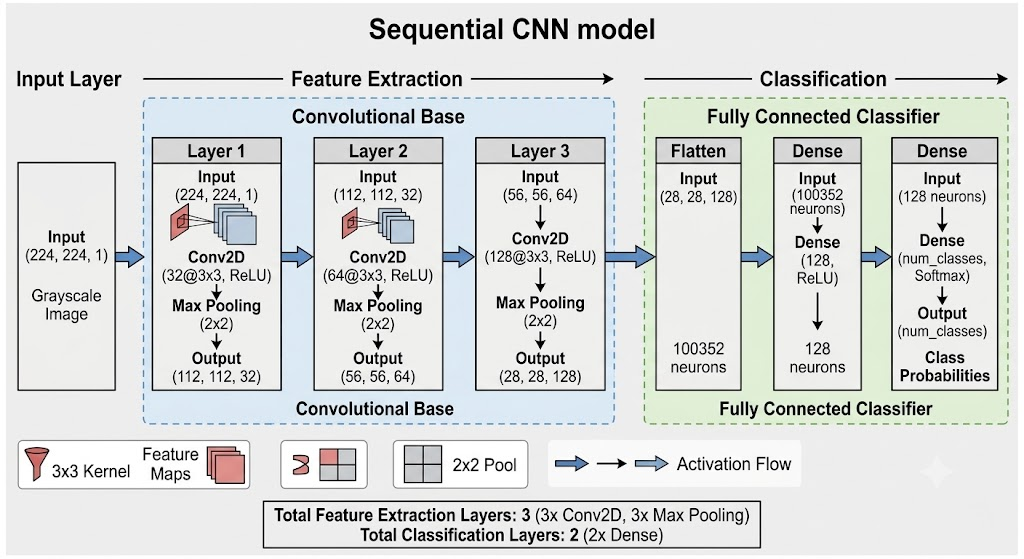
\includegraphics[width=0.95\linewidth]{media/cnn-arch.jpeg}
  \caption{ Architecture of the custom CNN model}
  \label{fig:cnnarch}
\end{figure*}

\subsection{Transfer Learning with MobileNetV2}

To overcome the limitations of training deep networks on a relatively small dataset, as illustreated in \cref{fig:mobilenetv2transfer}, transfer learning was employed using MobileNetV2 pre-trained on the ImageNet dataset.

The convolutional backbone of MobileNetV2 was initialized with pre-trained weights and frozen during training. A custom classification head consisting of a Global Average Pooling layer, Dropout layer, and Softmax output layer was added to adapt the model to the herbal plant classification task.

Early stopping was employed to prevent overfitting by monitoring validation loss during training. The transfer learning model was trained for up to 20 epochs and evaluated on the held-out test set.

% Figure 7: MobileNetV2 transfer learning architecture
\begin{figure*}[t]
  \centering
  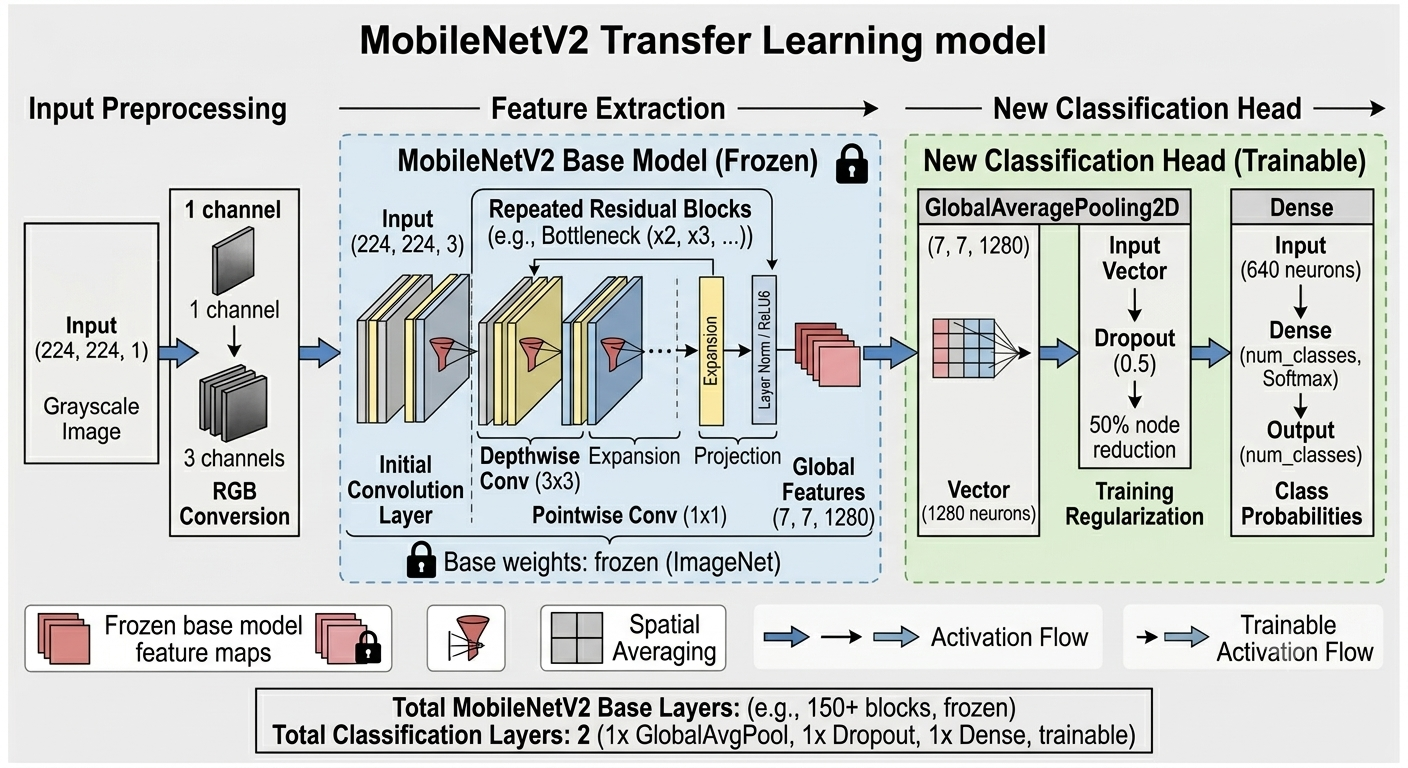
\includegraphics[width=0.95\linewidth]{media/mobilenetv2-transfer-learning.png}
  \caption{MobileNetV2 transfer learning architecture}
  \label{fig:mobilenetv2transfer}
\end{figure*}
